% lintrans - The linear transformation visualizer
% Copyright (C) 2021-2022 D. Dyson (DoctorDalek1963)

% This program is licensed under GNU GPLv3, available here:
% <https://www.gnu.org/licenses/gpl-3.0.html>

\documentclass[../main.tex]{subfiles}

\begin{document}

One of the topics in the A Level Further Maths course is linear transformations, as represented by matrices. This is a topic all about how vectors move and get transformed in the plane. It's a topic that lends itself exceedingly well to visualization, but students often find it hard to visualize this themselves, and there is a considerable lack of good tools to provide visual intuition on the subject. There is the YouTube series \textit{Essence of Linear Algebra} by 3blue1brown\cite{essence-of-linear-algebra}, which is excellent, but I couldn't find any good interactive visualizations.

My solution is to develop a desktop application that will allow the user to define $2 \times 2$ matrices and view these matrices and compositions thereof as linear transformations of a 2D plane. This will give students a way to get to grips with linear transformations in a more hands-on way, and will give teachers the ability to easily and visually show concepts like the determinant and invariant lines.

\subsection{Computational Approach\label{subsection:analysis:computational-approach}}

This solution is particularly well suited to a computational approach since it is entirely focussed on visualizing transformations, which require complex mathematics to properly display. It will also have lots of settings to allow the user to configure aspects of the visualization. As previously mentioned, visualizing transformations in one's own head is difficult, so a piece of software to do it would be very valuable to teachers and learners, but current solutions are considerably lacking.

My solution will make use of abstraction by allowing the user to define a set of matrices which they can use in expressions. This allows them to use a matrix multiple times and they don't have to keep track of any of the numbers. All the actual processing and mathematics happens behind the scenes and the user never has to worry about it - they just compose their defined matrices into transformations. This abstraction allows the user to focus on exploring the transformations themselves without having to do any actual computations. This will make learning the subject much easier, as they will able to gain a visual intuition for linear transformations without worrying about computation until after they've built up that intuition.

I will also employ decomposition and modularization by breaking the project down into many smaller parts, such as one module to keep track of defined matrices, one module to validate and parse matrix expressions, one module for the main GUI, as well as sub-modules for the widgets and dialog boxes, etc. This decomposition allows for simpler project design, easier code maintenance (since module coupling is kept to a minimum, so bugs are isolated in their modules), inheritance of classes to reduce code repetition, and unit testing to inform development. I also intend this unit testing to be automated using GitHub Actions.

Selection will also be used widely in the application. The GUI will provide many settings for visualization, and these settings will need to be checked when rendering the transformation. For example, the user will have the option to render the determinant, so I will need to check this setting on every render cycle and only render the determinant parallelogram if the user has enabled that option. The app will have many options for visualization, which will be useful in learning, but if all these options were being rendered at the same time, then there would be too much information for the user to properly process, so I will let the user configure these display options to their liking and only render the things they want to be rendered.

Validation will also be prevalent because the matrix expressions will need to follow a strict format, which will be validated. The buttons to render and animate the matrix will only be clickable when the given expression is valid, so I will need to check this and update the buttons every time the text in the text box is changed. I will also need to parse matrix expressions so that I can evaluate them properly. All this validation ensures that crashes due to malformed input are practically impossible, and makes the user's life easier since they don't need to worry about if their input is in the right format - the app will tell them.

I will also make use of iteration, primarily in animation. I will have to re-calculate positions and values to render everything for every frame of the animation and this will likely be done with a simple \texttt{for} loop. A \texttt{for} loop will allow me to just loop over every frame and use the counter variable as a way to measure how far through the animation we are on each frame. This is preferable to a \texttt{while} loop, since that would require me to keep track of which frame we're on with a separate variable.

Finally, the core of the application is visualization, so that will definitely be used a lot. I will have to calculate positions of points and lines based on given matrices, and when animating, I will also have to calculate these matrices based on the current frame. Then I will have to use the rendering capabilities of the GUI framework that I choose to render these calculated points and lines onto a widget, which will form the viewport of the main GUI. I may also have to convert between coordinate systems. I will have the origin in the middle with positive $x$ going to the right and positive $y$ going up, but I may need to convert that to standard computer graphics coordinates with the origin in the top left, positive $x$ going to the right, and positive $y$ going down. This visualization of linear transformations is the core component of the app and is the primary feature, so it is incredibly important.

\subsection{Stakeholders\label{subsection:analysis:stakeholders}}

Stakeholders for my app include A Level Further Maths students and teachers, who learn and teach linear transformations respectively. They will be able to provide useful input as to what they would like to see in the app, and they can provide feedback on what they like and what I can add or improve. I already know from experience that linear transformations are tricky to visualize and a computer-based visualization would be useful. My stakeholders agreed with this. Many teachers said that a desktop app that could render and animate linear transformations would be useful in a classroom environment and students said that it would be helpful to have something that they could play around with at home and use to get to grips with matrices and linear transformations.

Some teachers also suggested that it would be useful to have an option to save and load sets of matrices. This would allow them to have a single save file containing some matrices, and then just load this file to use for demonstrations in the classroom. This would probably be quite easy to implement. I could just wrap all the relevant information into one object and use Python's \texttt{pickle} module to save the binary data to a file, and then load this data back into the app in a similar way.

My stakeholders agreed that being able to see incremental animation - where, for example, we apply matrix $\mathbf{A}$ to the current scene, pause, and then apply matrix $\mathbf{B}$ - would be beneficial. This would be a good demonstration of matrix multiplication being non-commutative. $\mathbf{AB}$ is not always equal to $\mathbf{BA}$. Being able to see this in terms of animating linear transformations would be good for learning.

They also agreed that a tutorial on using the software would be useful, so I plan to implement this through an online written tutorial hosted with GitHub Pages, and perhaps a video tutorial as well. This would make the app much easier to use for people who have never seen it before. It wouldn't be a lesson on the maths itself, just a guide on how to use the software.

\subsection{Research on existing solutions\label{subsection:analysis:research-on-existing-solutions}}

There are actually quite a few web apps designed to help visualize 2D linear transformations but many of them are hard to use and lacking many features.

\subsubsection{MIT \enquote{Matrix Vector} Mathlet\label{subsubsection:analysis:mit-mathlet-matrix-vector}}

\begin{wrapfigure}{R}{0.5\linewidth}
	\vspace{-1em}
	\centering
	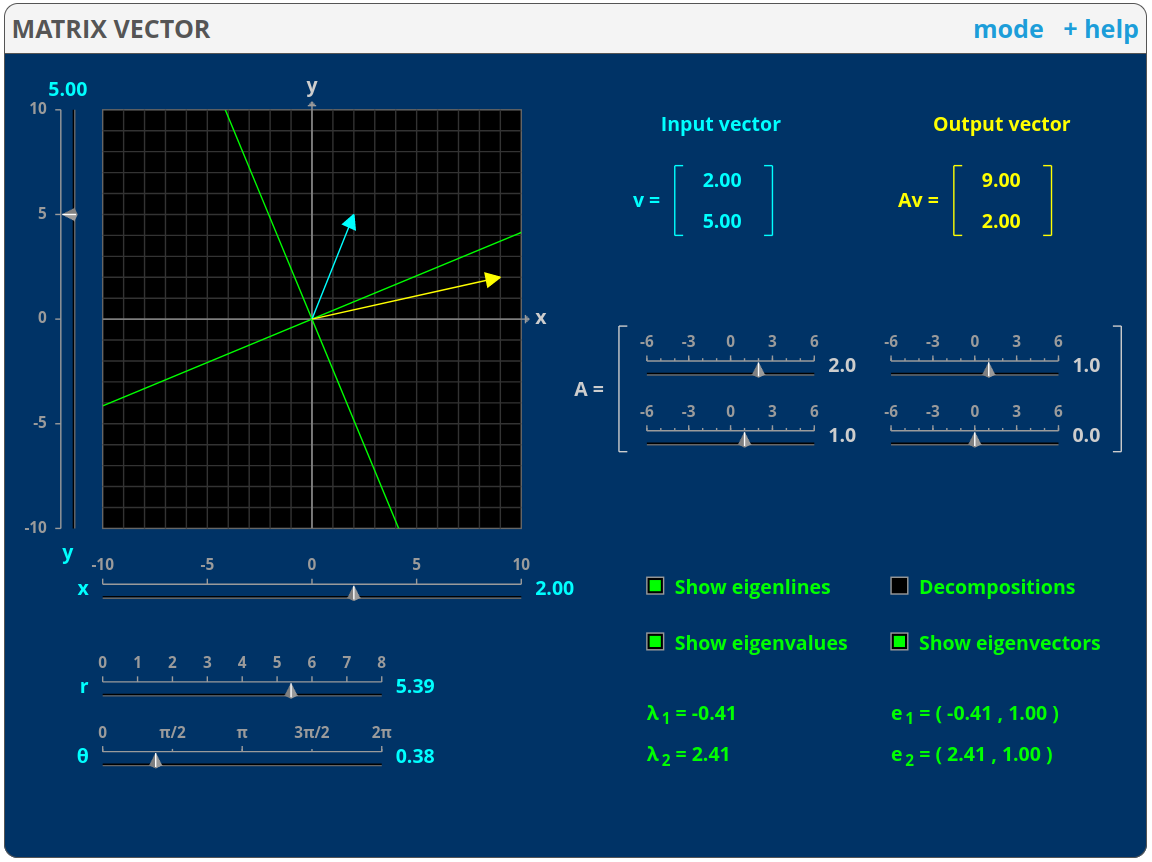
\includegraphics[width=\linewidth]{mit-mathlet-matrix-vector}
	\caption{The MIT \enquote{Matrix Vector} Mathlet}
	\label{fig:mit-mathlet-matrix-vector}
	\vspace{-1em}
\end{wrapfigure}

Arguably the best app that I found was an MIT \enquote{Mathlet} - a simple web app designed to help visualize a maths concept. This one is called \enquote{Matrix Vector}\cite{mit-mathlet-matrix-vector} and allows the user to drag an input vector around the plane and see the corresponding output vector, transformed by a matrix that the user can define, although this definition is finicky since it involves sliders rather than keyboard input.

This app fails in two crucial ways in my opinion. It doesn't show the basis vectors or let the user drag them around, and the user can only define and therefore visualize a single matrix at once. This second problem was common among every solution I found, so I won't mention it again, but it is a big issue in my opinion and my app will allow for multiple matrices. I like the idea of having a draggable input vector and rendering its output, so I will probably have this feature in my app, but I also want the ability to define multiple matrices and be able to drag the basis vectors to visually define a matrix. Being able to drag the basis vectors will help build intuition, so I think this would greatly benefit the app.

However, in the comments on this Mathlet, a user called \enquote{David~S.~Bruce} suggested that the Mathlet should display the basis vectors, to which a user called \enquote{hrm} (who I assume to be the \enquote{H.~Miller} to whom the copyright of the whole website is accredited) replied saying that this Mathlet is primarily focussed on eigenvectors, that it is perhaps badly named, and that displaying the basis vectors \enquote{would make a good focus for a second Mathlet about $2 \times 2$ matrices}. This Mathlet does not exist. But I do like the idea of showing the eigenvectors and eigenlines, so I will definitely have that in my app. Showing the invariant lines or lack thereof will help with learning, since these are often hard to visualize.

\subsubsection{Linear Transformation Visualizer\label{subsubsection:analysis:shad-io-matvis}}

\begin{wrapfigure}{L}{0.5\linewidth}
	\vspace{-1em}
	\centering
	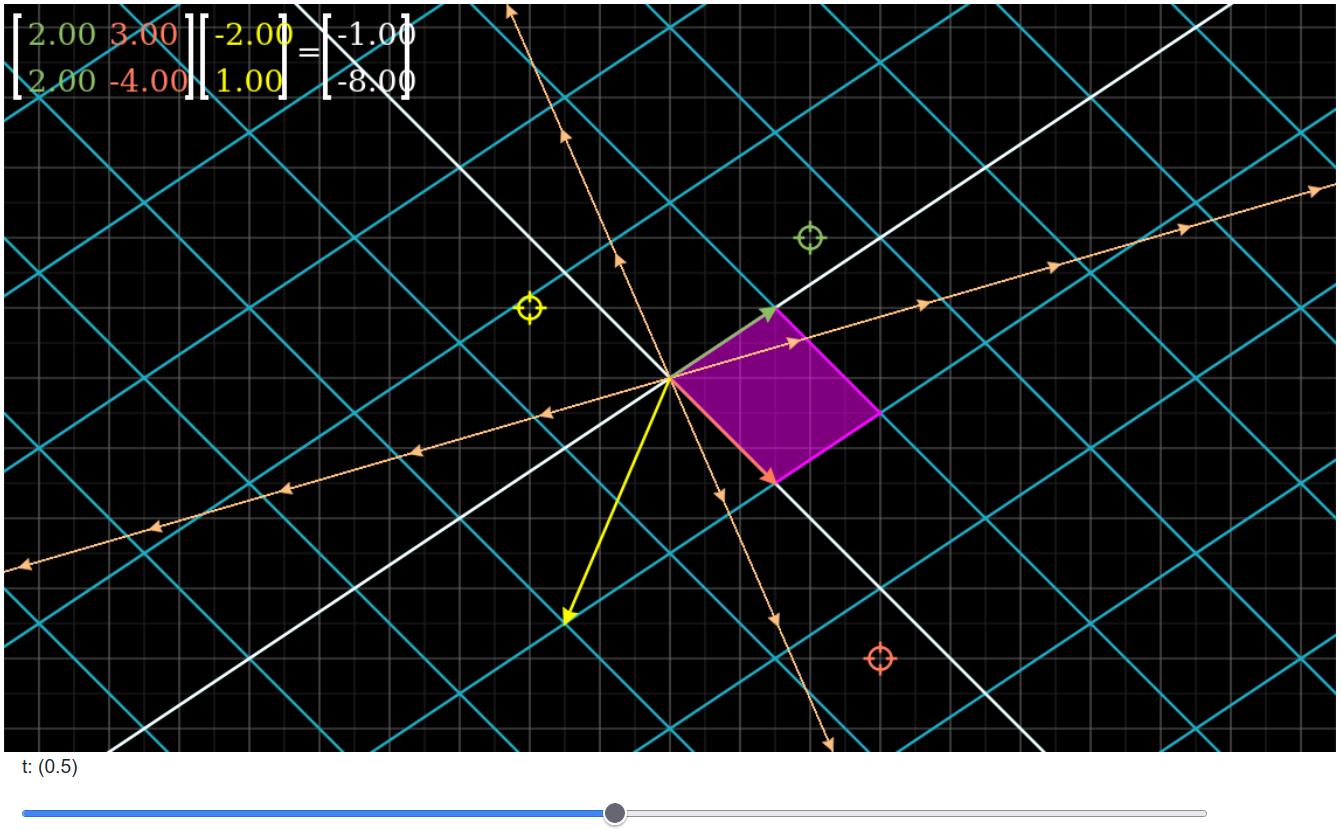
\includegraphics[width=\linewidth]{shad-io-matvis}
	\caption{\enquote{Linear Transformation Visualizer} halfway through an animation}
	\label{fig:shad-io-matvis}
	\vspace{-1em}
\end{wrapfigure}

Another web app that I found was one simply called \enquote{Linear Transformation Visualizer} by Shad~Sharma\cite{shad-io-matvis}. This one was similarly inspired by 3blue1brown's YouTube series. This app has the ability to render input and output vectors and eigenlines, but it can also render the determinant parallelogram; it allows the user to drag the basis vectors; and it has the option to snap vectors to the background grid, which is quite useful. It also implements a simple form of animation where the tips of the vectors move in straight lines from where they start to where they end, and the animation is controlled by dragging a slider labelled $t$. This isn't particularly intuitive.

I really like the vectors snapping to the grid, the input and output vectors, and rendering the determinant. This app also renders positive and negative determinants in different colours, which is really nice - I intend to use that idea in my own app, since it helps create understanding about negative determinants in terms of orientation changes. However, I think that the animation system here is flawed and not very easy to use. My animation will likely be a button, which just triggers an animation, rather than a slider. I also don't like the way vector dragging is handled. If you click anywhere on the grid, then the closest vector target (the final position of the target's associated vector) snaps to that location. I think it would be more intuitive to have to drag the vector from its current location to where you want it. This was also a problem with the MIT Mathlet.

\subsubsection{Desmos app\label{subsubsection:analysis:desmos-2d-linear-transformation}}

\begin{wrapfigure}{R}{0.5\linewidth}
	\vspace{-1em}
	\centering
	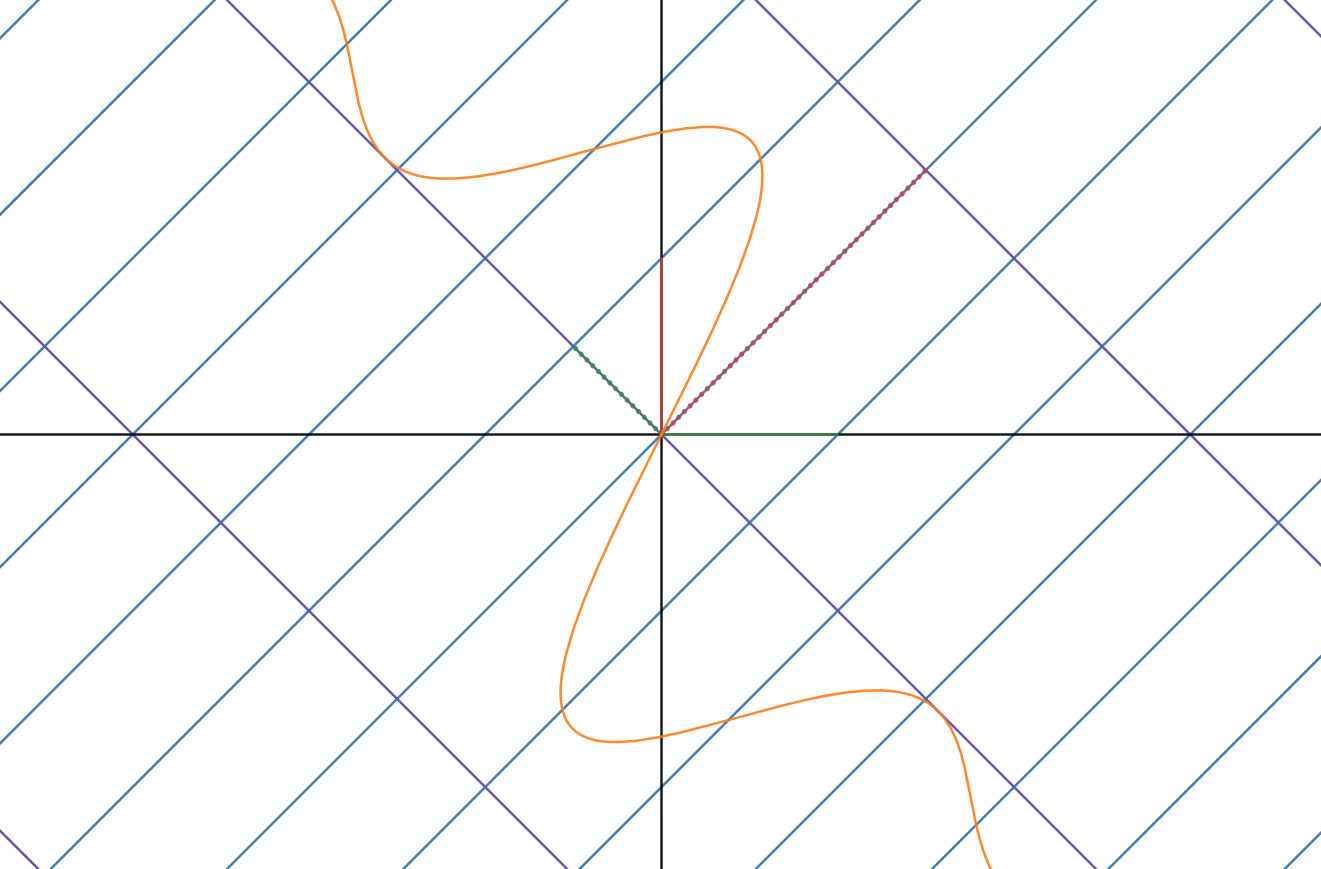
\includegraphics[width=\linewidth]{desmos-2d-linear-transformation}
	\caption{The Desmos app halfway through an animation, rendering $f(x) = \frac{\sin^2 x}{x}$ in orange}
	\label{fig:desmos-2d-linear-transformation}
	\vspace{-1em}
\end{wrapfigure}

One of the solutions I found was a Desmos app\cite{desmos-2d-linear-transformation}, which was quite hard to use and arguably overcomplicated. Desmos is not designed for this kind of thing - it's designed to graph pure mathematical functions - and it shows here. However, this app brings some really interesting ideas to the table, mainly functions. This app allows you to define custom functions and view them before and after the transformation. This is achieved by treating the functions parametrically as the set of points $(t, f(t))$ and then transforming each coordinate by the given matrix to get a new coordinate.

Desmos does this for every point and then renders the resulting transformed function parametrically. This is a really interesting technique and idea, but I'm not going to use it in my app. I don't think arbitrary functions fit with the linearity of the whole app, and I don't think it's necessary. It's just overcomplicating things, and rendering it on a widget would be tricky, because I'd have to render every point myself, possibly using something like OpenGL. It's just not worth implementing.

Additionally, this Desmos app makes things quite hard to see. It's hard to tell where any of the vectors are - they just get lost in the sea of grid lines. This image also hides some of the extra information. For instance, this image doesn't show the original function $f(x) = \frac{\sin^2 x}{x}$, only the transformed version. This app easily gets quite cluttered. I will give my vectors arrowheads to make them easily identifiable amongst the grid lines.

\subsubsection{Visualizing Linear Transformations\label{subsubsection:analysis:geogebra-applet}}

\begin{wrapfigure}{L}{0.5\linewidth}
	\vspace{-1em}
	\centering
	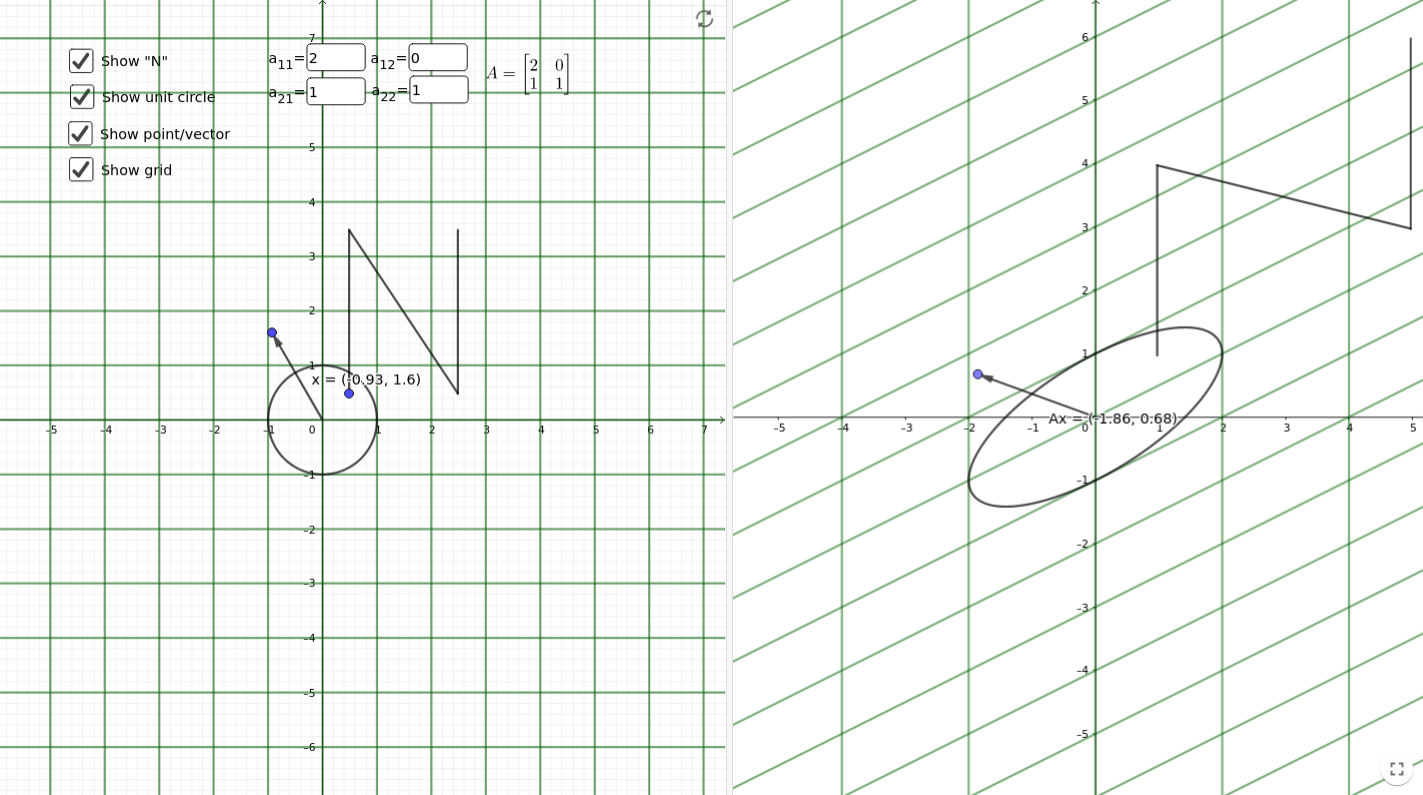
\includegraphics[width=\linewidth]{geogebra-applet}
	\caption{The GeoGebra applet rendering its default matrix}
	\label{fig:geogebra-applet}
	%\vspace{-1em}
\end{wrapfigure}

The last solution that I want to talk about is a GeoGebra applet simply titled \enquote{Visualizing Linear Transformations}\cite{geogebra-applet}. This applet has input and output vectors, original and transformed grid lines, a unit circle, and the letter N. It allows the user to define a matrix as 4 numbers and view the aforementioned N (which the user can translate to anywhere on the grid), the unit circle, the input/output vectors, and the grid lines. It also has the input vector snapping to integer coordinates, but that's a standard part of GeoGebra.

I've already talked about most of these features but the thing I wanted to talk about here is the N. I don't particularly want the letter N to be a prominent part of my own app, but I really like the idea of being able to define a custom polygon and see how that polygon gets transformed by a given transformation. I think that would really help with building intuition and it shouldn't be too hard to implement.

\subsection{Essential features\label{subsection:analysis:essential-features}}

The primary aim of this application is to visualize linear transformations, so this will obviously be the centre of the app and an essential feature. I will have a widget which can render a background grid and a second version of the grid, transformed according to a user-defined matrix expression. This is necessary because it is the entire purpose of the app. It's designed to visualize linear transformations and would be completely useless without this visual component. I will give the user the ability to render a custom matrix expression containing matrices they have previously defined, as well as reset the canvas to the default identity matrix transformation. This will obviously require an input box to enter the expression, a render button, a reset button, and various dialog boxes to define matrices in different ways. I want the user to be able to define a matrix as a set of 4 numbers, and by dragging the basis vectors $i$ and $j$. These dialogs will allow the user to define new matrices to be used in expressions, and having multiple ways to do it will make it easier, and will aid learning.

Another essential feature is animation. I want the user to be able to smoothly animate between matrices. I see two options for how this could work. If $\mathbf{C}$ is the matrix for the currently displayed transformation, and $\mathbf{T}$ is the matrix for the target transformation, then we could either animate from $\mathbf{C}$ to $\mathbf{T}$ or we could animate from $\mathbf{C}$ to $\mathbf{TC}$. I would probably call these transitional and applicative animation respectively. Perhaps I'll give the user the option to choose which animation method they want to use. Either way, animation is used in most of the alternative solutions that I found, and it's a great way to build intuition, by allowing students to watch the transformation happen in real time. Compared to simply rendering the transformations, animating them would profoundly benefit learning, and since that's the main aim of the project, I think animation is a necessary part of the app.

Something that I thought was a big problem in every alternative solution I found was the fact that the user could only visualize a single matrix at once. I see this as a fatal flaw and I will allow the user to define 25 different matrices (all capital letters except $\mathbf{I}$ for the identity matrix) and use all of them in expressions. This will allow teachers to define multiple matrices and then just change the expression to demonstrate different concepts rather than redefine a new transformation every time. It will also make things easier for students as it will allow them to visualize compositions of different matrix transformations without having to do any computations themselves.

Additionally, being able to show information on the currently displayed matrix is an essential tool for learning. Rendering things like the determinant parallelogram and the invariant lines of the transformation will greatly assist with learning and building understanding, so I think that having the option to render these attributes of the currently displayed transformation is necessary for success.

\subsection{Limitations\label{subsection:analysis:limitations}}

The main limitation in this app is likely to be drawing grid lines. Most transformations will be fine but in some cases, the app will be required to draw potentially thousands of grid lines on the canvas and this will probably cause noticeable lag, especially in the animations. I will have to artificially limit the number of grid lines that can be drawn on the screen. This won't look fantastic, because it means that the grid lines will only extend a certain distance from the origin, but it's an inherent limitation of computers. Perhaps if I was using a faster, compiled language like C++ rather than Python, this processing would happen faster and I could render more grid lines, but it's impossible to render all the grid lines and any implementation of this idea must limit them for performance.

An interesting limitation is that I don't think I'll implement panning. I suspect that I'll have to convert between coordinate systems and having the origin in the centre of the canvas will probably make the code much simpler. Also, linear transformations always leave the origin fixed, so always having it in the centre of the canvas seems thematically appropriate. Panning is certainly an option - the Desmos solution in \S\ref{subsubsection:analysis:desmos-2d-linear-transformation} and GeoGebra solution in \S\ref{subsubsection:analysis:geogebra-applet} both allow panning as a default part of Desmos and GeoGebra respectively, for example - but I don't think I'll implement it myself. I just don't think it's worth it.

I'm also not going to do any work with 3D linear transformations. 3D transformations are often harder to visualize and thus it would make sense to target them in an app like this, designed to help with learning and intuition, but 3D transformations are also harder to code. I would have to use a full graphics package rather than a simple widget, and I think it would be too much work for this project and I wouldn't be able to do it in the time frame. It's definitely a good idea, but I'm currently incapable of creating an app like that.

There are other limitations inherent to matrices. For instance, it's impossible to take an inverse of a singular matrix. There's nothing I can do about that without rewriting most of mathematics. Matrices can also only represent linear transformations. There's definitely a market for an app that could render any arbitrary transformation from $\mathbb{R}^2 \to \mathbb{R}^2$ - I know I'd want an app like that - but matrices can only represent linear transformations, so those are the only kind of transformations that I'll be looking at with this project.

\subsection{Hardware and software requirements\label{subsection:analysis:hardware-and-software-requirements}}

\subsubsection{Hardware\label{subsubsection:analysis:hardware}}

% TODO: Add size of final binary

Hardware requirements for the project are the same between the release and development environments and they're quite simple. I expect the app to require a processor with at least 1 GHz clock speed, \texttt{\$BINARY\_SIZE} free disk space, and about 1 GB of available RAM. The processor and RAM requirements are needed by the Python runtime and mainly by Qt5 - the GUI library I'll be using. The \texttt{\$BINARY\_SIZE} disk space is just for the executable binary that I'll compile for the public release. The code itself is less than 1 MB, but the compiled binary has to package all the dependencies and the entire CPython runtime to allow it to run on systems that don't have that, so the file size is much bigger.

I will also require that the user has a monitor that is at least $1920 \times 1080$ pixels in resolution. This isn't necessarily required, because the app will likely run in a smaller window, but a HD monitor is highly recommended. This allows the user to go fullscreen if they want to, and it gives them enough resolution to easily see everything in the app. A large, wall-mounted screen is also highly recommended for use in the classroom, although this is common among schools.

I will also require a keyboard with all standard Latin alphabet characters. This is because the matrices are defined as uppercase Latin letters. Any UK or US keyboard will suffice for this. The app will also require a mouse with at least one button. I don't intend to have right click do anything, so only the primary mouse button is required, although getting a single button mouse to actually work on modern computers is probably quite a challenge. A separate mouse is not strictly required - a laptop trackpad is equally sufficient.

\subsubsection{Software\label{subsubsection:analysis:software}}

% TODO: Find actual Windows version requirement

Software requirements differ slightly between release and development, although everything that the release environment requires is also required by the development environment. I will require a modern operating system - namely Windows 10 or later, macOS 10.9 \enquote{Mavericks}\footnote{Python 3.10 won't compile on any earlier versions of macOS\cite{python-3-10-downloads-page}} or later, or any modern Linux distro\footnote{Specifying a Linux version is practically impossible. Python 3.10 isn't available in many package repositories, but will compile on any modern distro. Qt5 is available in many package repositories and can be compiled on any \texttt{x86} or \texttt{x86\_64} generic Linux machine with \texttt{gcc} version 5 or later\cite{qt5-linux-build-dependencies}}. Basically, it just requires an operating system that is compatible with Python 3.10 and Qt5, since I'll be using these in the project. Of course, Qt5 will need to be installed on the user's computer, although it's standard pretty much everywhere these days.

Python 3.10 won't actually be required for the end user, because I will be compiling the app into a stand-alone binary executable for release, and this binary will contain the required Python runtime and dependencies. However, if the user wishes to download and run the source code themself, then they will need Python 3.10 and the package dependencies: \texttt{numpy}, \texttt{nptyping}, and \texttt{pyqt5}. These can be automatically installed with the command \texttt{python -m pip install -r requirements.txt} from the root of the repository. \texttt{numpy} is a maths library that allows for fast matrix maths; \texttt{nptyping} is used by \texttt{mypy} for type-checking and isn't actually a runtime dependency but the imports in the \texttt{typing} module fail if it's not installed at runtime; and \texttt{pyqt5} is a library that just allows interop between Python and Qt5, which is originally a C++ library.

In the development environment, I use PyCharm for actually writing my code, and I use a virtual environment to isolate my project dependencies. There are also some development dependencies listed in the file \texttt{dev\_requirements.txt}. They are: \texttt{mypy}, \texttt{pyqt5-stubs}, \texttt{flake8}, \texttt{pycodestyle}, \texttt{pydocstyle}, and \texttt{pytest}. \texttt{mypy} is a static type checker\footnote{Python has weak, dynamic typing with optional type annotations but \texttt{mypy} enforces these static type annotations}; \texttt{pyqt5-stubs} is a collection of type annotations for the PyQt5 API for \texttt{mypy} to use; \texttt{flake8}, \texttt{pycodestyle}, and \texttt{pydocstyle} are all linters; and \texttt{pytest} is a unit testing framework. I use these libraries to make sure my code is good quality and actually working properly during development.

\subsection{Success criteria\label{subsection:analysis:success-criteria}}

The main aim of the app is to help teach students about linear transformations. As such, the primary measure of success will be letting teachers get to grips with the app and then asking if they would use it in the classroom or recommend it to students to use at home.

Additionally, the app must fulfil some basic requirements:
\vspace{-0.3cm}
\begin{enumerate}
	\item\label{success-criterion:define-multiple-matrices} It must allow the user to define multiple matrices in at least two different ways (numerically and visually)
	\item\label{success-criterion:validate-arbitrary-matrix-expressions} It must be able to validate arbitrary matrix expressions
	\item\label{success-criterion:render-any-valid-expression} It must be able to render any valid matrix expression
	\item\label{success-criterion:animate-any-valid-expression} It must be able to animate any valid matrix expression
	\item\label{success-criterion:display-matrix-info} It must be able to display information about the currently rendered transformation (determinant, eigenlines, etc.)
	\item\label{success-criterion:save-and-load-sessions} It must be able to save and load sessions (defined matrices, display settings, etc.)
	\item\label{success-criterion:transform-polygons} It must allow the user to define and transform arbitrary polygons
\end{enumerate}

Defining multiple matrices is a feature that I thought was lacking from every other solution I researched, and I think it would make the app much easier to use, so I think it's necessary for success. Validating matrix expressions is necessary because if the user tries to render an expression that doesn't make sense, has an undefined matrix, or contains the inverse of a singular matrix, then we have to disallow that or else the app will crash.

Visualizing matrix expressions as linear transformations is the core part of the app, so basic rendering of them is definitely a requirement for success. Animating these expressions is also a pretty crucial part of the app, so I would consider this necessary for success. Displaying the information of a matrix transformation is also very useful for building understanding, so I would consider this needed to succeed.

Saving and loading isn't strictly necessary for success, but it is a standard part of many apps, so will likely be expected by users, and it will benefit the app by allowing teachers to plan lessons in advance and save the matrices they've defined for that lesson to be loaded later.

Transforming polygons is the lowest priority item on this list and will likely be implemented last, but it would definitely benefit learning. I wouldn't consider it necessary for success, but it would be very good to include, and it's certainly a feature that I want to have.

If the majority of teachers would use and/or recommend the app and it meets all of these points, then I will consider the app as a whole to be a success.

\end{document}
